% Options for packages loaded elsewhere
\PassOptionsToPackage{unicode}{hyperref}
\PassOptionsToPackage{hyphens}{url}
%
\documentclass[
]{article}
\usepackage{amsmath,amssymb}
\usepackage{iftex}
\ifPDFTeX
  \usepackage[T1]{fontenc}
  \usepackage[utf8]{inputenc}
  \usepackage{textcomp} % provide euro and other symbols
\else % if luatex or xetex
  \usepackage{unicode-math} % this also loads fontspec
  \defaultfontfeatures{Scale=MatchLowercase}
  \defaultfontfeatures[\rmfamily]{Ligatures=TeX,Scale=1}
\fi
\usepackage{lmodern}
\ifPDFTeX\else
  % xetex/luatex font selection
\fi
% Use upquote if available, for straight quotes in verbatim environments
\IfFileExists{upquote.sty}{\usepackage{upquote}}{}
\IfFileExists{microtype.sty}{% use microtype if available
  \usepackage[]{microtype}
  \UseMicrotypeSet[protrusion]{basicmath} % disable protrusion for tt fonts
}{}
\makeatletter
\@ifundefined{KOMAClassName}{% if non-KOMA class
  \IfFileExists{parskip.sty}{%
    \usepackage{parskip}
  }{% else
    \setlength{\parindent}{0pt}
    \setlength{\parskip}{6pt plus 2pt minus 1pt}}
}{% if KOMA class
  \KOMAoptions{parskip=half}}
\makeatother
\usepackage{xcolor}
\usepackage[margin=1in]{geometry}
\usepackage{color}
\usepackage{fancyvrb}
\newcommand{\VerbBar}{|}
\newcommand{\VERB}{\Verb[commandchars=\\\{\}]}
\DefineVerbatimEnvironment{Highlighting}{Verbatim}{commandchars=\\\{\}}
% Add ',fontsize=\small' for more characters per line
\usepackage{framed}
\definecolor{shadecolor}{RGB}{248,248,248}
\newenvironment{Shaded}{\begin{snugshade}}{\end{snugshade}}
\newcommand{\AlertTok}[1]{\textcolor[rgb]{0.94,0.16,0.16}{#1}}
\newcommand{\AnnotationTok}[1]{\textcolor[rgb]{0.56,0.35,0.01}{\textbf{\textit{#1}}}}
\newcommand{\AttributeTok}[1]{\textcolor[rgb]{0.13,0.29,0.53}{#1}}
\newcommand{\BaseNTok}[1]{\textcolor[rgb]{0.00,0.00,0.81}{#1}}
\newcommand{\BuiltInTok}[1]{#1}
\newcommand{\CharTok}[1]{\textcolor[rgb]{0.31,0.60,0.02}{#1}}
\newcommand{\CommentTok}[1]{\textcolor[rgb]{0.56,0.35,0.01}{\textit{#1}}}
\newcommand{\CommentVarTok}[1]{\textcolor[rgb]{0.56,0.35,0.01}{\textbf{\textit{#1}}}}
\newcommand{\ConstantTok}[1]{\textcolor[rgb]{0.56,0.35,0.01}{#1}}
\newcommand{\ControlFlowTok}[1]{\textcolor[rgb]{0.13,0.29,0.53}{\textbf{#1}}}
\newcommand{\DataTypeTok}[1]{\textcolor[rgb]{0.13,0.29,0.53}{#1}}
\newcommand{\DecValTok}[1]{\textcolor[rgb]{0.00,0.00,0.81}{#1}}
\newcommand{\DocumentationTok}[1]{\textcolor[rgb]{0.56,0.35,0.01}{\textbf{\textit{#1}}}}
\newcommand{\ErrorTok}[1]{\textcolor[rgb]{0.64,0.00,0.00}{\textbf{#1}}}
\newcommand{\ExtensionTok}[1]{#1}
\newcommand{\FloatTok}[1]{\textcolor[rgb]{0.00,0.00,0.81}{#1}}
\newcommand{\FunctionTok}[1]{\textcolor[rgb]{0.13,0.29,0.53}{\textbf{#1}}}
\newcommand{\ImportTok}[1]{#1}
\newcommand{\InformationTok}[1]{\textcolor[rgb]{0.56,0.35,0.01}{\textbf{\textit{#1}}}}
\newcommand{\KeywordTok}[1]{\textcolor[rgb]{0.13,0.29,0.53}{\textbf{#1}}}
\newcommand{\NormalTok}[1]{#1}
\newcommand{\OperatorTok}[1]{\textcolor[rgb]{0.81,0.36,0.00}{\textbf{#1}}}
\newcommand{\OtherTok}[1]{\textcolor[rgb]{0.56,0.35,0.01}{#1}}
\newcommand{\PreprocessorTok}[1]{\textcolor[rgb]{0.56,0.35,0.01}{\textit{#1}}}
\newcommand{\RegionMarkerTok}[1]{#1}
\newcommand{\SpecialCharTok}[1]{\textcolor[rgb]{0.81,0.36,0.00}{\textbf{#1}}}
\newcommand{\SpecialStringTok}[1]{\textcolor[rgb]{0.31,0.60,0.02}{#1}}
\newcommand{\StringTok}[1]{\textcolor[rgb]{0.31,0.60,0.02}{#1}}
\newcommand{\VariableTok}[1]{\textcolor[rgb]{0.00,0.00,0.00}{#1}}
\newcommand{\VerbatimStringTok}[1]{\textcolor[rgb]{0.31,0.60,0.02}{#1}}
\newcommand{\WarningTok}[1]{\textcolor[rgb]{0.56,0.35,0.01}{\textbf{\textit{#1}}}}
\usepackage{graphicx}
\makeatletter
\def\maxwidth{\ifdim\Gin@nat@width>\linewidth\linewidth\else\Gin@nat@width\fi}
\def\maxheight{\ifdim\Gin@nat@height>\textheight\textheight\else\Gin@nat@height\fi}
\makeatother
% Scale images if necessary, so that they will not overflow the page
% margins by default, and it is still possible to overwrite the defaults
% using explicit options in \includegraphics[width, height, ...]{}
\setkeys{Gin}{width=\maxwidth,height=\maxheight,keepaspectratio}
% Set default figure placement to htbp
\makeatletter
\def\fps@figure{htbp}
\makeatother
\setlength{\emergencystretch}{3em} % prevent overfull lines
\providecommand{\tightlist}{%
  \setlength{\itemsep}{0pt}\setlength{\parskip}{0pt}}
\setcounter{secnumdepth}{-\maxdimen} % remove section numbering
\ifLuaTeX
  \usepackage{selnolig}  % disable illegal ligatures
\fi
\usepackage{bookmark}
\IfFileExists{xurl.sty}{\usepackage{xurl}}{} % add URL line breaks if available
\urlstyle{same}
\hypersetup{
  pdftitle={jan2021},
  hidelinks,
  pdfcreator={LaTeX via pandoc}}

\title{jan2021}
\author{}
\date{\vspace{-2.5em}2024-10-27}

\begin{document}
\maketitle

\section{1. Graphical Models (6 p) - Using the IC
Algorithn}\label{graphical-models-6-p---using-the-ic-algorithn}

\subsection{Overview of the IC
Algorithm}\label{overview-of-the-ic-algorithm}

\paragraph{The IC algorithm consists of three main
steps:}\label{the-ic-algorithm-consists-of-three-main-steps}

\begin{enumerate}
\def\labelenumi{\arabic{enumi}.}
\tightlist
\item
  \emph{Skeleton Discovery}: Construct an undirected graph that
  represents dependencies between variables.
\item
  \emph{Edge Orientation with V-Structures}: Identify causal directions
  by finding V-structures (patterns where A--\textgreater{} B
  \textless-- C with no edge between A and C).
\item
  \emph{Propagation of Orientation}: Further orient edges using rules to
  avoid cycles and preserve conditional independencies.
\end{enumerate}

\begin{Shaded}
\begin{Highlighting}[]
\FunctionTok{library}\NormalTok{(bnlearn)}

\FunctionTok{data}\NormalTok{(}\StringTok{"lizards"}\NormalTok{)}

\NormalTok{lizardsnet}\OtherTok{\textless{}{-}}\FunctionTok{model2network}\NormalTok{(}\StringTok{"[Species][Diameter|Species][Height|Species]"}\NormalTok{) }\CommentTok{\# True DAG}
\FunctionTok{plot}\NormalTok{(lizardsnet)}
\end{Highlighting}
\end{Shaded}

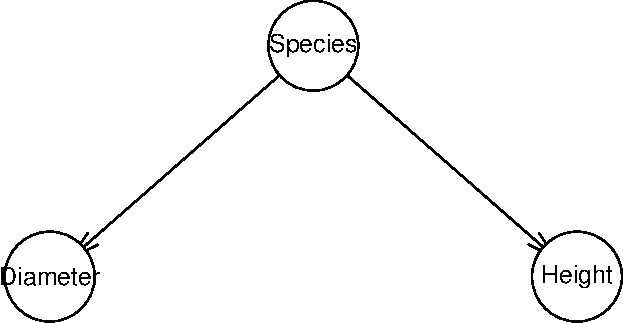
\includegraphics{jan2021_files/figure-latex/unnamed-chunk-1-1.pdf}

\begin{Shaded}
\begin{Highlighting}[]
\FunctionTok{plot}\NormalTok{(}\FunctionTok{cpdag}\NormalTok{(lizardsnet)) }\CommentTok{\# Plot the true pattern}
\end{Highlighting}
\end{Shaded}

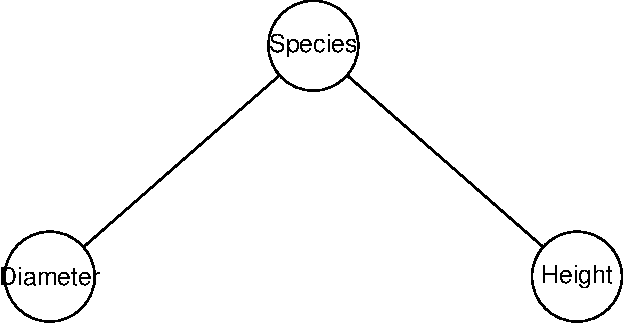
\includegraphics{jan2021_files/figure-latex/unnamed-chunk-1-2.pdf}

\begin{Shaded}
\begin{Highlighting}[]
\CommentTok{\# Independence if p{-}value is \textgreater{} 0.05}

\CommentTok{\# Skeleton discovery}
\FunctionTok{ci.test}\NormalTok{(}\AttributeTok{x =} \StringTok{"Diameter"}\NormalTok{, }\AttributeTok{y =} \StringTok{"Species"}\NormalTok{, }\AttributeTok{data =}\NormalTok{ lizards)  }\CommentTok{\# Keep edge D{-}S. (Not independent given empty set)}
\end{Highlighting}
\end{Shaded}

\begin{verbatim}
## 
##  Mutual Information (disc.)
## 
## data:  Diameter ~ Species  
## mi = 12.606, df = 1, p-value = 0.0003845
## alternative hypothesis: true value is greater than 0
\end{verbatim}

\begin{Shaded}
\begin{Highlighting}[]
\FunctionTok{ci.test}\NormalTok{(}\AttributeTok{x =} \StringTok{"Diameter"}\NormalTok{, }\AttributeTok{y =} \StringTok{"Height"}\NormalTok{, }\AttributeTok{data =}\NormalTok{ lizards)   }\CommentTok{\# Remove edge D{-}H. (Independent given empty set)}
\end{Highlighting}
\end{Shaded}

\begin{verbatim}
## 
##  Mutual Information (disc.)
## 
## data:  Diameter ~ Height  
## mi = 0.60771, df = 1, p-value = 0.4357
## alternative hypothesis: true value is greater than 0
\end{verbatim}

\begin{Shaded}
\begin{Highlighting}[]
\FunctionTok{ci.test}\NormalTok{(}\AttributeTok{x =} \StringTok{"Height"}\NormalTok{, }\AttributeTok{y =} \StringTok{"Species"}\NormalTok{, }\AttributeTok{data =}\NormalTok{ lizards)    }\CommentTok{\# Keep edge H{-}S. (Not independent given empty set)}
\end{Highlighting}
\end{Shaded}

\begin{verbatim}
## 
##  Mutual Information (disc.)
## 
## data:  Height ~ Species  
## mi = 10.405, df = 1, p-value = 0.001257
## alternative hypothesis: true value is greater than 0
\end{verbatim}

\begin{Shaded}
\begin{Highlighting}[]
\CommentTok{\# The skeleton now looks like this:}
\NormalTok{currmod }\OtherTok{=} \FunctionTok{model2network}\NormalTok{(}\StringTok{"[Species][Diameter|Species][Height|Species]"}\NormalTok{)}
\FunctionTok{plot}\NormalTok{(}\FunctionTok{cpdag}\NormalTok{(currmod))}

\CommentTok{\# Edge Orientation with V{-}Structures}
\CommentTok{\# Investigate non adjacent vairables}
\FunctionTok{ci.test}\NormalTok{(}\AttributeTok{x =} \StringTok{"Diameter"}\NormalTok{, }\AttributeTok{y =} \StringTok{"Height"}\NormalTok{, }\AttributeTok{z =} \StringTok{"Species"}\NormalTok{, }\AttributeTok{data =}\NormalTok{ lizards) }\CommentTok{\# D and H are independent given S}
\end{Highlighting}
\end{Shaded}

\begin{verbatim}
## 
##  Mutual Information (disc.)
## 
## data:  Diameter ~ Height | Species
## mi = 2.0256, df = 2, p-value = 0.3632
## alternative hypothesis: true value is greater than 0
\end{verbatim}

\begin{Shaded}
\begin{Highlighting}[]
\CommentTok{\# Since this test showed that D and H are conditionally independent, }
\CommentTok{\# we choose S as an unsheilded collider: D {-}{-}\textgreater{} S \textless{}{-}{-} H}


\FunctionTok{plot}\NormalTok{(}\FunctionTok{model2network}\NormalTok{(}\StringTok{"[Diameter][Height][Species|Diameter:Height]"}\NormalTok{))}
\end{Highlighting}
\end{Shaded}

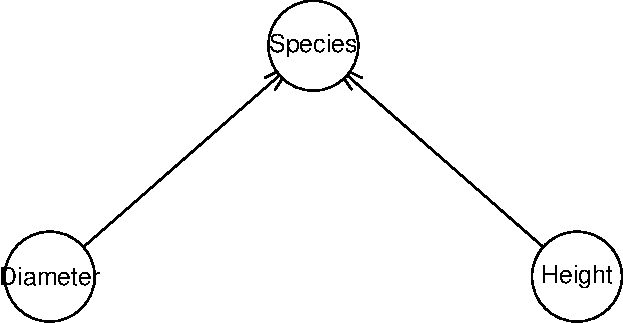
\includegraphics{jan2021_files/figure-latex/unnamed-chunk-1-3.pdf}

\section{2. Hidden Markov Models (7 p)}\label{hidden-markov-models-7-p}

\begin{Shaded}
\begin{Highlighting}[]
\FunctionTok{library}\NormalTok{(bnlearn)}
\FunctionTok{library}\NormalTok{(gRain)}
\end{Highlighting}
\end{Shaded}

\begin{verbatim}
## Loading required package: gRbase
\end{verbatim}

\begin{verbatim}
## 
## Attaching package: 'gRbase'
\end{verbatim}

\begin{verbatim}
## The following objects are masked from 'package:bnlearn':
## 
##     ancestors, children, nodes, parents
\end{verbatim}

\begin{Shaded}
\begin{Highlighting}[]
\NormalTok{hmm }\OtherTok{\textless{}{-}} \FunctionTok{model2network}\NormalTok{(}\StringTok{"[z0][x0|z0][z1|z0][x1|z1][z2|z1][x2|z2][z3|z2][x3|z3]"}\NormalTok{) }\CommentTok{\# True DAG}

\NormalTok{states }\OtherTok{=} \FunctionTok{c}\NormalTok{(}\StringTok{"1"}\NormalTok{,}\StringTok{"2"}\NormalTok{,}\StringTok{"3"}\NormalTok{,}\StringTok{"4"}\NormalTok{,}\StringTok{"5"}\NormalTok{,}\StringTok{"6"}\NormalTok{,}\StringTok{"7"}\NormalTok{,}\StringTok{"8"}\NormalTok{,}\StringTok{"9"}\NormalTok{,}\StringTok{"10"}\NormalTok{)}
\NormalTok{symbols }\OtherTok{=} \FunctionTok{c}\NormalTok{(}\StringTok{"1"}\NormalTok{,}\StringTok{"2"}\NormalTok{,}\StringTok{"3"}\NormalTok{,}\StringTok{"4"}\NormalTok{,}\StringTok{"5"}\NormalTok{,}\StringTok{"6"}\NormalTok{,}\StringTok{"7"}\NormalTok{,}\StringTok{"8"}\NormalTok{,}\StringTok{"9"}\NormalTok{,}\StringTok{"10"}\NormalTok{)}

\NormalTok{transitionProb }\OtherTok{=} \FunctionTok{matrix}\NormalTok{(}\DecValTok{0}\NormalTok{,}\AttributeTok{nrow =} \DecValTok{10}\NormalTok{, }\AttributeTok{ncol =} \DecValTok{10}\NormalTok{)}
\ControlFlowTok{for}\NormalTok{ (j }\ControlFlowTok{in} \DecValTok{1}\SpecialCharTok{:}\DecValTok{10}\NormalTok{) \{}
\NormalTok{  transitionProb[j,j] }\OtherTok{=} \FloatTok{0.5}
\NormalTok{  transitionProb[j,j}\SpecialCharTok{\%\%}\DecValTok{10} \SpecialCharTok{+}\DecValTok{1}\NormalTok{ ] }\OtherTok{=} \FloatTok{0.5}
\NormalTok{\}}

\NormalTok{emissionProb }\OtherTok{=} \FunctionTok{matrix}\NormalTok{(}\DecValTok{0}\NormalTok{,}\AttributeTok{nrow =} \DecValTok{10}\NormalTok{, }\AttributeTok{ncol =} \DecValTok{10}\NormalTok{)}
\ControlFlowTok{for}\NormalTok{ (j }\ControlFlowTok{in} \DecValTok{1}\SpecialCharTok{:}\DecValTok{10}\NormalTok{) \{}
  \ControlFlowTok{for}\NormalTok{ (i }\ControlFlowTok{in} \DecValTok{1}\SpecialCharTok{:}\DecValTok{5}\NormalTok{) \{}
\NormalTok{    emissionProb[(j}\SpecialCharTok{+}\NormalTok{i}\DecValTok{{-}4}\NormalTok{)}\SpecialCharTok{\%\%}\DecValTok{10}\SpecialCharTok{+}\DecValTok{1}\NormalTok{,j] }\OtherTok{=} \FloatTok{0.2}
\NormalTok{  \}}
\NormalTok{\}}

\DocumentationTok{\#\#\#\#\#\# Hidden states \#\#\#\#\#\#}
\NormalTok{cptZ0 }\OtherTok{=} \FunctionTok{rep}\NormalTok{(}\FloatTok{0.1}\NormalTok{,}\DecValTok{10}\NormalTok{)}
\FunctionTok{dim}\NormalTok{(cptZ0) }\OtherTok{=} \FunctionTok{c}\NormalTok{(}\DecValTok{10}\NormalTok{)}
\FunctionTok{dimnames}\NormalTok{(cptZ0) }\OtherTok{=} \FunctionTok{list}\NormalTok{(states)}

\NormalTok{cptZ1 }\OtherTok{=}\NormalTok{ transitionProb}
\FunctionTok{dim}\NormalTok{(cptZ1) }\OtherTok{=} \FunctionTok{c}\NormalTok{(}\DecValTok{10}\NormalTok{,}\DecValTok{10}\NormalTok{)}
\FunctionTok{dimnames}\NormalTok{(cptZ1) }\OtherTok{=} \FunctionTok{list}\NormalTok{(}\StringTok{"z1"} \OtherTok{=}\NormalTok{ states, }\StringTok{"z0"} \OtherTok{=}\NormalTok{ states)}


\NormalTok{cptZ2 }\OtherTok{=}\NormalTok{ transitionProb}
\FunctionTok{dim}\NormalTok{(cptZ2) }\OtherTok{=} \FunctionTok{c}\NormalTok{(}\DecValTok{10}\NormalTok{,}\DecValTok{10}\NormalTok{)}
\FunctionTok{dimnames}\NormalTok{(cptZ2) }\OtherTok{=} \FunctionTok{list}\NormalTok{(}\StringTok{"z2"} \OtherTok{=}\NormalTok{ states, }\StringTok{"z1"} \OtherTok{=}\NormalTok{ states)}

\NormalTok{cptZ3 }\OtherTok{=}\NormalTok{ transitionProb}
\FunctionTok{dim}\NormalTok{(cptZ3) }\OtherTok{=} \FunctionTok{c}\NormalTok{(}\DecValTok{10}\NormalTok{,}\DecValTok{10}\NormalTok{)}
\FunctionTok{dimnames}\NormalTok{(cptZ3) }\OtherTok{=} \FunctionTok{list}\NormalTok{(}\StringTok{"z3"} \OtherTok{=}\NormalTok{ states, }\StringTok{"z2"} \OtherTok{=}\NormalTok{ states)}
\DocumentationTok{\#\#\#\#\#\#\#\#\#\#\#\#\#\#\#\#\#\#\#\#\#\#\#\#\#\#\#\#\#}

\DocumentationTok{\#\#\#\#\#\# observed states \#\#\#\#\#\#}
\NormalTok{cptX0 }\OtherTok{=}\NormalTok{ emissionProb}
\FunctionTok{dim}\NormalTok{(cptX0) }\OtherTok{=} \FunctionTok{c}\NormalTok{(}\DecValTok{10}\NormalTok{,}\DecValTok{10}\NormalTok{)}
\FunctionTok{dimnames}\NormalTok{(cptX0) }\OtherTok{=} \FunctionTok{list}\NormalTok{(}\StringTok{"x0"} \OtherTok{=}\NormalTok{ symbols, }\StringTok{"z0"} \OtherTok{=}\NormalTok{ states)}

\NormalTok{cptX1 }\OtherTok{=}\NormalTok{ emissionProb}
\FunctionTok{dim}\NormalTok{(cptX1) }\OtherTok{=} \FunctionTok{c}\NormalTok{(}\DecValTok{10}\NormalTok{,}\DecValTok{10}\NormalTok{)}
\FunctionTok{dimnames}\NormalTok{(cptX1) }\OtherTok{=} \FunctionTok{list}\NormalTok{(}\StringTok{"x1"} \OtherTok{=}\NormalTok{ symbols, }\StringTok{"z1"} \OtherTok{=}\NormalTok{ states)}

\NormalTok{cptX2 }\OtherTok{=}\NormalTok{ emissionProb}
\FunctionTok{dim}\NormalTok{(cptX2) }\OtherTok{=} \FunctionTok{c}\NormalTok{(}\DecValTok{10}\NormalTok{,}\DecValTok{10}\NormalTok{)}
\FunctionTok{dimnames}\NormalTok{(cptX2) }\OtherTok{=} \FunctionTok{list}\NormalTok{(}\StringTok{"x2"} \OtherTok{=}\NormalTok{ symbols, }\StringTok{"z2"} \OtherTok{=}\NormalTok{ states)}

\NormalTok{cptX3 }\OtherTok{=}\NormalTok{ emissionProb}
\FunctionTok{dim}\NormalTok{(cptX3) }\OtherTok{=} \FunctionTok{c}\NormalTok{(}\DecValTok{10}\NormalTok{,}\DecValTok{10}\NormalTok{)}
\FunctionTok{dimnames}\NormalTok{(cptX3) }\OtherTok{=} \FunctionTok{list}\NormalTok{(}\StringTok{"x3"} \OtherTok{=}\NormalTok{ symbols, }\StringTok{"z3"} \OtherTok{=}\NormalTok{ states)}
\DocumentationTok{\#\#\#\#\#\#\#\#\#\#\#\#\#\#\#\#\#\#\#\#\#\#\#\#\#\#\#\#\#}

\NormalTok{nodes }\OtherTok{=} \FunctionTok{c}\NormalTok{(}\StringTok{"z0"}\NormalTok{, }\StringTok{"z1"}\NormalTok{, }\StringTok{"z2"}\NormalTok{, }\StringTok{"z3"}\NormalTok{, }\StringTok{"x0"}\NormalTok{, }\StringTok{"x1"}\NormalTok{, }\StringTok{"x2"}\NormalTok{, }\StringTok{"x3"}\NormalTok{)}
\NormalTok{hmmfit }\OtherTok{=} \FunctionTok{custom.fit}\NormalTok{(hmm, }\FunctionTok{list}\NormalTok{(}\AttributeTok{z0=}\NormalTok{cptZ0, }\AttributeTok{z1=}\NormalTok{cptZ1, }\AttributeTok{z2=}\NormalTok{cptZ2, }\AttributeTok{z3=}\NormalTok{cptZ3, }\AttributeTok{x0=}\NormalTok{cptX0, }\AttributeTok{x1=}\NormalTok{cptX1, }\AttributeTok{x2=}\NormalTok{cptX2, }\AttributeTok{x3=}\NormalTok{cptX3))}
\NormalTok{compiledgrain }\OtherTok{=} \FunctionTok{compile}\NormalTok{(}\FunctionTok{as.grain}\NormalTok{(hmmfit))}


\FunctionTok{querygrain}\NormalTok{(}\FunctionTok{setEvidence}\NormalTok{(compiledgrain,}\AttributeTok{nodes =} \FunctionTok{c}\NormalTok{(}\StringTok{"x0"}\NormalTok{, }\StringTok{"x2"}\NormalTok{), }\AttributeTok{states =} \FunctionTok{c}\NormalTok{(}\StringTok{"1"}\NormalTok{,}\StringTok{"3"}\NormalTok{)), }\AttributeTok{nodes =} \StringTok{"z0"}\NormalTok{)}\SpecialCharTok{$}\NormalTok{z0}
\end{Highlighting}
\end{Shaded}

\begin{verbatim}
## z0
##     1     2     3     4     5     6     7     8     9    10 
## 0.125 0.375 0.500 0.000 0.000 0.000 0.000 0.000 0.000 0.000
\end{verbatim}

\begin{Shaded}
\begin{Highlighting}[]
\FunctionTok{querygrain}\NormalTok{(}\FunctionTok{setEvidence}\NormalTok{(compiledgrain,}\AttributeTok{nodes =} \FunctionTok{c}\NormalTok{(}\StringTok{"x0"}\NormalTok{, }\StringTok{"x2"}\NormalTok{), }\AttributeTok{states =} \FunctionTok{c}\NormalTok{(}\StringTok{"1"}\NormalTok{,}\StringTok{"3"}\NormalTok{)), }\AttributeTok{nodes =} \StringTok{"z1"}\NormalTok{)}\SpecialCharTok{$}\NormalTok{z1}
\end{Highlighting}
\end{Shaded}

\begin{verbatim}
## z1
##    1    2    3    4    5    6    7    8    9   10 
## 0.25 0.50 0.25 0.00 0.00 0.00 0.00 0.00 0.00 0.00
\end{verbatim}

\begin{Shaded}
\begin{Highlighting}[]
\FunctionTok{querygrain}\NormalTok{(}\FunctionTok{setEvidence}\NormalTok{(compiledgrain,}\AttributeTok{nodes =} \FunctionTok{c}\NormalTok{(}\StringTok{"x0"}\NormalTok{, }\StringTok{"x2"}\NormalTok{), }\AttributeTok{states =} \FunctionTok{c}\NormalTok{(}\StringTok{"1"}\NormalTok{,}\StringTok{"3"}\NormalTok{)), }\AttributeTok{nodes =} \StringTok{"z2"}\NormalTok{)}\SpecialCharTok{$}\NormalTok{z2}
\end{Highlighting}
\end{Shaded}

\begin{verbatim}
## z2
##     1     2     3     4     5     6     7     8     9    10 
## 0.500 0.375 0.125 0.000 0.000 0.000 0.000 0.000 0.000 0.000
\end{verbatim}

\begin{Shaded}
\begin{Highlighting}[]
\FunctionTok{querygrain}\NormalTok{(}\FunctionTok{setEvidence}\NormalTok{(compiledgrain,}\AttributeTok{nodes =} \FunctionTok{c}\NormalTok{(}\StringTok{"x0"}\NormalTok{, }\StringTok{"x2"}\NormalTok{), }\AttributeTok{states =} \FunctionTok{c}\NormalTok{(}\StringTok{"1"}\NormalTok{,}\StringTok{"3"}\NormalTok{)), }\AttributeTok{nodes =} \StringTok{"z3"}\NormalTok{)}\SpecialCharTok{$}\NormalTok{z3}
\end{Highlighting}
\end{Shaded}

\begin{verbatim}
## z3
##      1      2      3      4      5      6      7      8      9     10 
## 0.4375 0.2500 0.0625 0.0000 0.0000 0.0000 0.0000 0.0000 0.0000 0.2500
\end{verbatim}

\section{3. Reinforcement Learning (7
p)}\label{reinforcement-learning-7-p}

\begin{Shaded}
\begin{Highlighting}[]
\FunctionTok{set.seed}\NormalTok{(}\DecValTok{1234}\NormalTok{)}
\FunctionTok{library}\NormalTok{(ggplot2)}

\NormalTok{arrows }\OtherTok{\textless{}{-}} \FunctionTok{c}\NormalTok{(}\StringTok{"\^{}"}\NormalTok{, }\StringTok{"\textgreater{}"}\NormalTok{, }\StringTok{"v"}\NormalTok{, }\StringTok{"\textless{}"}\NormalTok{)}
\NormalTok{action\_deltas }\OtherTok{\textless{}{-}} \FunctionTok{list}\NormalTok{(}\FunctionTok{c}\NormalTok{(}\DecValTok{1}\NormalTok{,}\DecValTok{0}\NormalTok{), }\CommentTok{\# up}
                      \FunctionTok{c}\NormalTok{(}\DecValTok{0}\NormalTok{,}\DecValTok{1}\NormalTok{), }\CommentTok{\# right}
                      \FunctionTok{c}\NormalTok{(}\SpecialCharTok{{-}}\DecValTok{1}\NormalTok{,}\DecValTok{0}\NormalTok{), }\CommentTok{\# down}
                      \FunctionTok{c}\NormalTok{(}\DecValTok{0}\NormalTok{,}\SpecialCharTok{{-}}\DecValTok{1}\NormalTok{)) }\CommentTok{\# left}

\NormalTok{vis\_environment }\OtherTok{\textless{}{-}} \ControlFlowTok{function}\NormalTok{(}\AttributeTok{iterations=}\DecValTok{0}\NormalTok{, }\AttributeTok{epsilon =} \FloatTok{0.5}\NormalTok{, }\AttributeTok{alpha =} \FloatTok{0.1}\NormalTok{, }\AttributeTok{gamma =} \FloatTok{0.95}\NormalTok{, }\AttributeTok{beta =} \DecValTok{0}\NormalTok{)\{}

  
\NormalTok{  df }\OtherTok{\textless{}{-}} \FunctionTok{expand.grid}\NormalTok{(}\AttributeTok{x=}\DecValTok{1}\SpecialCharTok{:}\NormalTok{H,}\AttributeTok{y=}\DecValTok{1}\SpecialCharTok{:}\NormalTok{W)}
\NormalTok{  foo }\OtherTok{\textless{}{-}} \FunctionTok{mapply}\NormalTok{(}\ControlFlowTok{function}\NormalTok{(x,y) }\FunctionTok{ifelse}\NormalTok{(reward\_map[x,y] }\SpecialCharTok{==} \DecValTok{0}\NormalTok{,q\_table[x,y,}\DecValTok{1}\NormalTok{],}\ConstantTok{NA}\NormalTok{),df}\SpecialCharTok{$}\NormalTok{x,df}\SpecialCharTok{$}\NormalTok{y)}
\NormalTok{  df}\SpecialCharTok{$}\NormalTok{val1 }\OtherTok{\textless{}{-}} \FunctionTok{as.vector}\NormalTok{(}\FunctionTok{round}\NormalTok{(foo, }\DecValTok{2}\NormalTok{))}
\NormalTok{  foo }\OtherTok{\textless{}{-}} \FunctionTok{mapply}\NormalTok{(}\ControlFlowTok{function}\NormalTok{(x,y) }\FunctionTok{ifelse}\NormalTok{(reward\_map[x,y] }\SpecialCharTok{==} \DecValTok{0}\NormalTok{,q\_table[x,y,}\DecValTok{2}\NormalTok{],}\ConstantTok{NA}\NormalTok{),df}\SpecialCharTok{$}\NormalTok{x,df}\SpecialCharTok{$}\NormalTok{y)}
\NormalTok{  df}\SpecialCharTok{$}\NormalTok{val2 }\OtherTok{\textless{}{-}} \FunctionTok{as.vector}\NormalTok{(}\FunctionTok{round}\NormalTok{(foo, }\DecValTok{2}\NormalTok{))}
\NormalTok{  foo }\OtherTok{\textless{}{-}} \FunctionTok{mapply}\NormalTok{(}\ControlFlowTok{function}\NormalTok{(x,y) }\FunctionTok{ifelse}\NormalTok{(reward\_map[x,y] }\SpecialCharTok{==} \DecValTok{0}\NormalTok{,q\_table[x,y,}\DecValTok{3}\NormalTok{],}\ConstantTok{NA}\NormalTok{),df}\SpecialCharTok{$}\NormalTok{x,df}\SpecialCharTok{$}\NormalTok{y)}
\NormalTok{  df}\SpecialCharTok{$}\NormalTok{val3 }\OtherTok{\textless{}{-}} \FunctionTok{as.vector}\NormalTok{(}\FunctionTok{round}\NormalTok{(foo, }\DecValTok{2}\NormalTok{))}
\NormalTok{  foo }\OtherTok{\textless{}{-}} \FunctionTok{mapply}\NormalTok{(}\ControlFlowTok{function}\NormalTok{(x,y) }\FunctionTok{ifelse}\NormalTok{(reward\_map[x,y] }\SpecialCharTok{==} \DecValTok{0}\NormalTok{,q\_table[x,y,}\DecValTok{4}\NormalTok{],}\ConstantTok{NA}\NormalTok{),df}\SpecialCharTok{$}\NormalTok{x,df}\SpecialCharTok{$}\NormalTok{y)}
\NormalTok{  df}\SpecialCharTok{$}\NormalTok{val4 }\OtherTok{\textless{}{-}} \FunctionTok{as.vector}\NormalTok{(}\FunctionTok{round}\NormalTok{(foo, }\DecValTok{2}\NormalTok{))}
\NormalTok{  foo }\OtherTok{\textless{}{-}} \FunctionTok{mapply}\NormalTok{(}\ControlFlowTok{function}\NormalTok{(x,y) }
    \FunctionTok{ifelse}\NormalTok{(reward\_map[x,y] }\SpecialCharTok{==} \DecValTok{0}\NormalTok{,arrows[}\FunctionTok{GreedyPolicy}\NormalTok{(x,y)],reward\_map[x,y]),df}\SpecialCharTok{$}\NormalTok{x,df}\SpecialCharTok{$}\NormalTok{y)}
\NormalTok{  df}\SpecialCharTok{$}\NormalTok{val5 }\OtherTok{\textless{}{-}} \FunctionTok{as.vector}\NormalTok{(foo)}
\NormalTok{  foo }\OtherTok{\textless{}{-}} \FunctionTok{mapply}\NormalTok{(}\ControlFlowTok{function}\NormalTok{(x,y) }\FunctionTok{ifelse}\NormalTok{(reward\_map[x,y] }\SpecialCharTok{==} \DecValTok{0}\NormalTok{,}\FunctionTok{max}\NormalTok{(q\_table[x,y,]),}
                                     \FunctionTok{ifelse}\NormalTok{(reward\_map[x,y]}\SpecialCharTok{\textless{}}\DecValTok{0}\NormalTok{,}\ConstantTok{NA}\NormalTok{,reward\_map[x,y])),df}\SpecialCharTok{$}\NormalTok{x,df}\SpecialCharTok{$}\NormalTok{y)}
\NormalTok{  df}\SpecialCharTok{$}\NormalTok{val6 }\OtherTok{\textless{}{-}} \FunctionTok{as.vector}\NormalTok{(foo)}
  
  \FunctionTok{print}\NormalTok{(}\FunctionTok{ggplot}\NormalTok{(df,}\FunctionTok{aes}\NormalTok{(}\AttributeTok{x =}\NormalTok{ y,}\AttributeTok{y =}\NormalTok{ x)) }\SpecialCharTok{+}
          \FunctionTok{scale\_fill\_gradient}\NormalTok{(}\AttributeTok{low =} \StringTok{"white"}\NormalTok{, }\AttributeTok{high =} \StringTok{"green"}\NormalTok{, }\AttributeTok{na.value =} \StringTok{"red"}\NormalTok{, }\AttributeTok{name =} \StringTok{""}\NormalTok{) }\SpecialCharTok{+}
          \FunctionTok{geom\_tile}\NormalTok{(}\FunctionTok{aes}\NormalTok{(}\AttributeTok{fill=}\NormalTok{val6)) }\SpecialCharTok{+}
          \FunctionTok{geom\_text}\NormalTok{(}\FunctionTok{aes}\NormalTok{(}\AttributeTok{label =}\NormalTok{ val1),}\AttributeTok{size =} \DecValTok{4}\NormalTok{,}\AttributeTok{nudge\_y =}\NormalTok{ .}\DecValTok{35}\NormalTok{,}\AttributeTok{na.rm =} \ConstantTok{TRUE}\NormalTok{) }\SpecialCharTok{+}
          \FunctionTok{geom\_text}\NormalTok{(}\FunctionTok{aes}\NormalTok{(}\AttributeTok{label =}\NormalTok{ val2),}\AttributeTok{size =} \DecValTok{4}\NormalTok{,}\AttributeTok{nudge\_x =}\NormalTok{ .}\DecValTok{35}\NormalTok{,}\AttributeTok{na.rm =} \ConstantTok{TRUE}\NormalTok{) }\SpecialCharTok{+}
          \FunctionTok{geom\_text}\NormalTok{(}\FunctionTok{aes}\NormalTok{(}\AttributeTok{label =}\NormalTok{ val3),}\AttributeTok{size =} \DecValTok{4}\NormalTok{,}\AttributeTok{nudge\_y =} \SpecialCharTok{{-}}\NormalTok{.}\DecValTok{35}\NormalTok{,}\AttributeTok{na.rm =} \ConstantTok{TRUE}\NormalTok{) }\SpecialCharTok{+}
          \FunctionTok{geom\_text}\NormalTok{(}\FunctionTok{aes}\NormalTok{(}\AttributeTok{label =}\NormalTok{ val4),}\AttributeTok{size =} \DecValTok{4}\NormalTok{,}\AttributeTok{nudge\_x =} \SpecialCharTok{{-}}\NormalTok{.}\DecValTok{35}\NormalTok{,}\AttributeTok{na.rm =} \ConstantTok{TRUE}\NormalTok{) }\SpecialCharTok{+}
          \FunctionTok{geom\_text}\NormalTok{(}\FunctionTok{aes}\NormalTok{(}\AttributeTok{label =}\NormalTok{ val5),}\AttributeTok{size =} \DecValTok{10}\NormalTok{) }\SpecialCharTok{+}
          \FunctionTok{geom\_tile}\NormalTok{(}\AttributeTok{fill =} \StringTok{\textquotesingle{}transparent\textquotesingle{}}\NormalTok{, }\AttributeTok{colour =} \StringTok{\textquotesingle{}black\textquotesingle{}}\NormalTok{) }\SpecialCharTok{+} 
          \FunctionTok{ggtitle}\NormalTok{(}\FunctionTok{paste}\NormalTok{(}\StringTok{"Q{-}table after "}\NormalTok{,iterations,}\StringTok{" iterations}\SpecialCharTok{\textbackslash{}n}\StringTok{"}\NormalTok{,}
                        \StringTok{"(epsilon = "}\NormalTok{,epsilon,}\StringTok{", alpha = "}\NormalTok{,alpha,}\StringTok{"gamma = "}\NormalTok{,}
\NormalTok{                        gamma,}\StringTok{", beta = "}\NormalTok{,beta,}\StringTok{")"}\NormalTok{)) }\SpecialCharTok{+}
          \FunctionTok{theme}\NormalTok{(}\AttributeTok{plot.title =} \FunctionTok{element\_text}\NormalTok{(}\AttributeTok{hjust =} \FloatTok{0.5}\NormalTok{)) }\SpecialCharTok{+}
          \FunctionTok{scale\_x\_continuous}\NormalTok{(}\AttributeTok{breaks =} \FunctionTok{c}\NormalTok{(}\DecValTok{1}\SpecialCharTok{:}\NormalTok{W),}\AttributeTok{labels =} \FunctionTok{c}\NormalTok{(}\DecValTok{1}\SpecialCharTok{:}\NormalTok{W)) }\SpecialCharTok{+}
          \FunctionTok{scale\_y\_continuous}\NormalTok{(}\AttributeTok{breaks =} \FunctionTok{c}\NormalTok{(}\DecValTok{1}\SpecialCharTok{:}\NormalTok{H),}\AttributeTok{labels =} \FunctionTok{c}\NormalTok{(}\DecValTok{1}\SpecialCharTok{:}\NormalTok{H)))}

\NormalTok{\}}

\NormalTok{GreedyPolicy }\OtherTok{\textless{}{-}} \ControlFlowTok{function}\NormalTok{(x, y)\{}

\NormalTok{  q\_values }\OtherTok{=}\NormalTok{ q\_table[x, y, ]}
  
  \CommentTok{\# Find all actions with the maximum Q{-}value}
\NormalTok{  max\_actions }\OtherTok{=} \FunctionTok{which}\NormalTok{(q\_values }\SpecialCharTok{==} \FunctionTok{max}\NormalTok{(q\_values))}
  \ControlFlowTok{if}\NormalTok{ (}\FunctionTok{length}\NormalTok{(max\_actions) }\SpecialCharTok{==} \DecValTok{1}\NormalTok{) \{}
    \FunctionTok{return}\NormalTok{(max\_actions)}
\NormalTok{  \} }\ControlFlowTok{else}\NormalTok{ \{}
    \FunctionTok{return}\NormalTok{(}\FunctionTok{sample}\NormalTok{(max\_actions, }\DecValTok{1}\NormalTok{))}
\NormalTok{  \}}
  
\NormalTok{\}}

\NormalTok{EpsilonGreedyPolicy }\OtherTok{\textless{}{-}} \ControlFlowTok{function}\NormalTok{(x, y, epsilon)\{}

  \CommentTok{\# Your code here.}
  \ControlFlowTok{if}\NormalTok{ (}\FunctionTok{runif}\NormalTok{(}\DecValTok{1}\NormalTok{) }\SpecialCharTok{\textless{}}\NormalTok{ epsilon) \{}
    \FunctionTok{return}\NormalTok{ (}\FunctionTok{sample}\NormalTok{(}\DecValTok{1}\SpecialCharTok{:}\DecValTok{4}\NormalTok{,}\DecValTok{1}\NormalTok{))}
\NormalTok{  \} }\ControlFlowTok{else}\NormalTok{ \{}
    \FunctionTok{return}\NormalTok{ (}\FunctionTok{GreedyPolicy}\NormalTok{(x,y))}
\NormalTok{  \}}
\NormalTok{\}}

\NormalTok{transition\_model }\OtherTok{\textless{}{-}} \ControlFlowTok{function}\NormalTok{(x, y, action, beta)\{}

\NormalTok{  delta }\OtherTok{\textless{}{-}} \FunctionTok{sample}\NormalTok{(}\SpecialCharTok{{-}}\DecValTok{1}\SpecialCharTok{:}\DecValTok{1}\NormalTok{, }\AttributeTok{size =} \DecValTok{1}\NormalTok{, }\AttributeTok{prob =} \FunctionTok{c}\NormalTok{(}\FloatTok{0.5}\SpecialCharTok{*}\NormalTok{beta,}\DecValTok{1}\SpecialCharTok{{-}}\NormalTok{beta,}\FloatTok{0.5}\SpecialCharTok{*}\NormalTok{beta))}
\NormalTok{  final\_action }\OtherTok{\textless{}{-}}\NormalTok{ ((action }\SpecialCharTok{+}\NormalTok{ delta }\SpecialCharTok{+} \DecValTok{3}\NormalTok{) }\SpecialCharTok{\%\%} \DecValTok{4}\NormalTok{) }\SpecialCharTok{+} \DecValTok{1}
\NormalTok{  foo }\OtherTok{\textless{}{-}} \FunctionTok{c}\NormalTok{(x,y) }\SpecialCharTok{+} \FunctionTok{unlist}\NormalTok{(action\_deltas[final\_action])}
\NormalTok{  foo }\OtherTok{\textless{}{-}} \FunctionTok{pmax}\NormalTok{(}\FunctionTok{c}\NormalTok{(}\DecValTok{1}\NormalTok{,}\DecValTok{1}\NormalTok{),}\FunctionTok{pmin}\NormalTok{(foo,}\FunctionTok{c}\NormalTok{(H,W)))}
  
  \FunctionTok{return}\NormalTok{ (foo)}
\NormalTok{\}}

\NormalTok{q\_learning }\OtherTok{\textless{}{-}} \ControlFlowTok{function}\NormalTok{(start\_state, }\AttributeTok{epsilon =} \FloatTok{0.5}\NormalTok{, }\AttributeTok{alpha =} \FloatTok{0.1}\NormalTok{, }\AttributeTok{gamma =} \FloatTok{0.95}\NormalTok{, }
                       \AttributeTok{beta =} \DecValTok{0}\NormalTok{, }\AttributeTok{tr =} \DecValTok{1}\NormalTok{)\{}
\NormalTok{  Q }\OtherTok{=}\NormalTok{ start\_state}
\NormalTok{  x }\OtherTok{=}\NormalTok{ Q[}\DecValTok{1}\NormalTok{]}
\NormalTok{  y }\OtherTok{=}\NormalTok{ Q[}\DecValTok{2}\NormalTok{]}
\NormalTok{  episode\_correction }\OtherTok{=} \DecValTok{0}
\NormalTok{  ite }\OtherTok{=} \DecValTok{0}
  \ControlFlowTok{repeat}\NormalTok{\{}
    
    \CommentTok{\# Follow policy, execute action, get reward.}
\NormalTok{    action }\OtherTok{=} \FunctionTok{EpsilonGreedyPolicy}\NormalTok{(x,y,epsilon}\SpecialCharTok{*}\NormalTok{tr) }\CommentTok{\# follow policy}
\NormalTok{    next\_state }\OtherTok{=} \FunctionTok{transition\_model}\NormalTok{(x,y,action,beta) }\CommentTok{\# excecute action}
\NormalTok{    reward }\OtherTok{=}\NormalTok{ reward\_map[next\_state[}\DecValTok{1}\NormalTok{],next\_state[}\DecValTok{2}\NormalTok{]] }\CommentTok{\# get reward}
    
    \CommentTok{\# Q{-}table update.}
\NormalTok{    correction }\OtherTok{=} \FunctionTok{ifelse}\NormalTok{(reward }\SpecialCharTok{==} \DecValTok{0}\NormalTok{, }\SpecialCharTok{{-}}\DecValTok{1}\NormalTok{, reward) }\SpecialCharTok{+}\NormalTok{ gamma }\SpecialCharTok{*} \FunctionTok{max}\NormalTok{(q\_table[next\_state[}\DecValTok{1}\NormalTok{],next\_state[}\DecValTok{2}\NormalTok{],])}\SpecialCharTok{{-}}\NormalTok{q\_table[x,y,action]}
\NormalTok{    q\_table[x,y,action] }\OtherTok{\textless{}\textless{}{-}}\NormalTok{ q\_table[x,y,action] }\SpecialCharTok{+}\NormalTok{ alpha }\SpecialCharTok{*}\NormalTok{ (correction}\SpecialCharTok{*}\NormalTok{tr)}
\NormalTok{    episode\_correction }\OtherTok{=}\NormalTok{ episode\_correction }\SpecialCharTok{+}\NormalTok{ correction}\SpecialCharTok{*}\NormalTok{tr}
    
\NormalTok{    x }\OtherTok{=}\NormalTok{ next\_state[}\DecValTok{1}\NormalTok{]}
\NormalTok{    y }\OtherTok{=}\NormalTok{ next\_state[}\DecValTok{2}\NormalTok{]}
    
    \ControlFlowTok{if}\NormalTok{(reward}\SpecialCharTok{!=}\DecValTok{0}\NormalTok{)}
      \CommentTok{\# End episode.}
      \FunctionTok{return}\NormalTok{ (}\FunctionTok{c}\NormalTok{(reward }\SpecialCharTok{{-}}\NormalTok{ ite,episode\_correction))}
    \ControlFlowTok{else}
\NormalTok{      ite }\OtherTok{=}\NormalTok{ ite }\SpecialCharTok{+} \DecValTok{1}
\NormalTok{  \}}
  
\NormalTok{\}}

\NormalTok{SARSA }\OtherTok{\textless{}{-}} \ControlFlowTok{function}\NormalTok{(start\_state, }\AttributeTok{epsilon =} \FloatTok{0.5}\NormalTok{, }\AttributeTok{alpha =} \FloatTok{0.1}\NormalTok{, }\AttributeTok{gamma =} \FloatTok{0.95}\NormalTok{, }\AttributeTok{beta =} \DecValTok{0}\NormalTok{)\{}
\NormalTok{  Q }\OtherTok{=}\NormalTok{ start\_state}
\NormalTok{  x }\OtherTok{=}\NormalTok{ Q[}\DecValTok{1}\NormalTok{]}
\NormalTok{  y }\OtherTok{=}\NormalTok{ Q[}\DecValTok{2}\NormalTok{]}
\NormalTok{  episode\_correction }\OtherTok{=} \DecValTok{0}
\NormalTok{  ite }\OtherTok{=} \DecValTok{0}
  \CommentTok{\#next\_action = EpsilonGreedyPolicy(x,y,epsilon) \# follow policy}
  \ControlFlowTok{repeat}\NormalTok{\{}

    \CommentTok{\# S A R S A}
    \CommentTok{\# Follow policy, execute action, get reward.}
\NormalTok{    action }\OtherTok{=} \FunctionTok{EpsilonGreedyPolicy}\NormalTok{(x,y,epsilon)}
\NormalTok{    next\_state }\OtherTok{=} \FunctionTok{transition\_model}\NormalTok{(x,y,action,beta) }\CommentTok{\# excecute action}
\NormalTok{    reward }\OtherTok{=}\NormalTok{ reward\_map[next\_state[}\DecValTok{1}\NormalTok{],next\_state[}\DecValTok{2}\NormalTok{]] }\CommentTok{\# get reward}
\NormalTok{    next\_action }\OtherTok{=} \FunctionTok{EpsilonGreedyPolicy}\NormalTok{(next\_state[}\DecValTok{1}\NormalTok{],next\_state[}\DecValTok{2}\NormalTok{],epsilon) }\CommentTok{\# follow policy}

    \CommentTok{\# Q{-}table update.}
\NormalTok{    correction }\OtherTok{=} \FunctionTok{ifelse}\NormalTok{(reward}\SpecialCharTok{==}\DecValTok{0}\NormalTok{,}\SpecialCharTok{{-}}\DecValTok{1}\NormalTok{,reward) }\SpecialCharTok{+}\NormalTok{ gamma }\SpecialCharTok{*}\NormalTok{ (q\_table[next\_state[}\DecValTok{1}\NormalTok{],next\_state[}\DecValTok{2}\NormalTok{],next\_action])}\SpecialCharTok{{-}}\NormalTok{q\_table[x,y,action]}
\NormalTok{    q\_table[x,y,action] }\OtherTok{\textless{}\textless{}{-}}\NormalTok{ q\_table[x,y,action] }\SpecialCharTok{+}\NormalTok{ alpha }\SpecialCharTok{*}\NormalTok{ (correction)}
\NormalTok{    episode\_correction }\OtherTok{=}\NormalTok{ episode\_correction }\SpecialCharTok{+}\NormalTok{ correction}

\NormalTok{    x }\OtherTok{=}\NormalTok{ next\_state[}\DecValTok{1}\NormalTok{]}
\NormalTok{    y }\OtherTok{=}\NormalTok{ next\_state[}\DecValTok{2}\NormalTok{]}

    \ControlFlowTok{if}\NormalTok{(reward}\SpecialCharTok{!=}\DecValTok{0}\NormalTok{) \{}
      \CommentTok{\# End episode.}
      \FunctionTok{return}\NormalTok{ (}\FunctionTok{c}\NormalTok{(reward }\SpecialCharTok{{-}}\NormalTok{ ite, episode\_correction))}
\NormalTok{    \}}
    \ControlFlowTok{else}\NormalTok{ \{}
\NormalTok{      ite }\OtherTok{=}\NormalTok{ ite }\SpecialCharTok{+} \DecValTok{1}
\NormalTok{    \}}
\NormalTok{  \}}

\NormalTok{\}}



\NormalTok{SARSASA }\OtherTok{\textless{}{-}} \ControlFlowTok{function}\NormalTok{(start\_state, }\AttributeTok{epsilon =} \FloatTok{0.5}\NormalTok{, }\AttributeTok{alpha =} \FloatTok{0.1}\NormalTok{, }\AttributeTok{gamma =} \FloatTok{0.95}\NormalTok{, }\AttributeTok{beta =} \DecValTok{0}\NormalTok{)\{}
\NormalTok{  Q }\OtherTok{=}\NormalTok{ start\_state}
\NormalTok{  x }\OtherTok{=}\NormalTok{ Q[}\DecValTok{1}\NormalTok{]}
\NormalTok{  y }\OtherTok{=}\NormalTok{ Q[}\DecValTok{2}\NormalTok{]}
\NormalTok{  episode\_correction }\OtherTok{=} \DecValTok{0}
\NormalTok{  ite }\OtherTok{=} \DecValTok{0}
  \CommentTok{\#next\_action = EpsilonGreedyPolicy(x,y,epsilon) \# follow policy}
  \ControlFlowTok{repeat}\NormalTok{\{}

    \CommentTok{\# S A R S A}
    \CommentTok{\# Follow policy, execute action, get reward.}
\NormalTok{    action }\OtherTok{=} \FunctionTok{EpsilonGreedyPolicy}\NormalTok{(x,y,epsilon)}
\NormalTok{    next\_state }\OtherTok{=} \FunctionTok{transition\_model}\NormalTok{(x,y,action,beta) }\CommentTok{\# excecute action}
\NormalTok{    reward }\OtherTok{=}\NormalTok{ reward\_map[next\_state[}\DecValTok{1}\NormalTok{],next\_state[}\DecValTok{2}\NormalTok{]] }\CommentTok{\# get reward}
\NormalTok{    next\_action }\OtherTok{=} \FunctionTok{EpsilonGreedyPolicy}\NormalTok{(next\_state[}\DecValTok{1}\NormalTok{],next\_state[}\DecValTok{2}\NormalTok{],epsilon) }\CommentTok{\# follow policy}
    
    \CommentTok{\# S A}
    \ControlFlowTok{if}\NormalTok{ (reward}\SpecialCharTok{!=}\DecValTok{0}\NormalTok{) \{}
\NormalTok{      next\_next\_state }\OtherTok{=} \FunctionTok{transition\_model}\NormalTok{(next\_state[}\DecValTok{1}\NormalTok{],next\_state[}\DecValTok{2}\NormalTok{],next\_action,beta) }\CommentTok{\# excecute action}
\NormalTok{      next\_reward }\OtherTok{=}\NormalTok{ reward\_map[next\_next\_state[}\DecValTok{1}\NormalTok{],next\_next\_state[}\DecValTok{2}\NormalTok{]] }\CommentTok{\# get reward}
\NormalTok{      next\_next\_action }\OtherTok{=} \FunctionTok{EpsilonGreedyPolicy}\NormalTok{(next\_next\_state[}\DecValTok{1}\NormalTok{],next\_next\_state[}\DecValTok{2}\NormalTok{],epsilon)}
    
\NormalTok{      correction }\OtherTok{=} \FunctionTok{ifelse}\NormalTok{(next\_reward}\SpecialCharTok{==}\DecValTok{0}\NormalTok{,}\SpecialCharTok{{-}}\DecValTok{1}\NormalTok{,next\_reward) }\SpecialCharTok{+}\NormalTok{ gamma }\SpecialCharTok{*}\NormalTok{ (q\_table[next\_next\_state[}\DecValTok{1}\NormalTok{],next\_next\_state[}\DecValTok{2}\NormalTok{],}
\NormalTok{                                                                            next\_next\_action])}\SpecialCharTok{{-}}\NormalTok{q\_table[next\_state[}\DecValTok{1}\NormalTok{],next\_state[}\DecValTok{2}\NormalTok{],next\_action]}
\NormalTok{      q\_table[x,y,action] }\OtherTok{\textless{}\textless{}{-}}\NormalTok{ q\_table[x,y,action] }\SpecialCharTok{+}\NormalTok{ alpha }\SpecialCharTok{*}\NormalTok{ (correction)}
\NormalTok{      episode\_correction }\OtherTok{=}\NormalTok{ episode\_correction }\SpecialCharTok{+}\NormalTok{ correction      }
\NormalTok{    \} }

    \CommentTok{\# Q{-}table update.}
\NormalTok{    correction }\OtherTok{=} \FunctionTok{ifelse}\NormalTok{(reward}\SpecialCharTok{==}\DecValTok{0}\NormalTok{,}\SpecialCharTok{{-}}\DecValTok{1}\NormalTok{,reward) }\SpecialCharTok{+}\NormalTok{ gamma }\SpecialCharTok{*}\NormalTok{ (q\_table[next\_state[}\DecValTok{1}\NormalTok{],next\_state[}\DecValTok{2}\NormalTok{],next\_action])}\SpecialCharTok{{-}}\NormalTok{q\_table[x,y,action]}
\NormalTok{    q\_table[x,y,action] }\OtherTok{\textless{}\textless{}{-}}\NormalTok{ q\_table[x,y,action] }\SpecialCharTok{+}\NormalTok{ alpha }\SpecialCharTok{*}\NormalTok{ (correction)}
\NormalTok{    episode\_correction }\OtherTok{=}\NormalTok{ episode\_correction }\SpecialCharTok{+}\NormalTok{ correction}

\NormalTok{    x }\OtherTok{=}\NormalTok{ next\_state[}\DecValTok{1}\NormalTok{]}
\NormalTok{    y }\OtherTok{=}\NormalTok{ next\_state[}\DecValTok{2}\NormalTok{]}

    \ControlFlowTok{if}\NormalTok{(reward}\SpecialCharTok{!=}\DecValTok{0}\NormalTok{) \{}
      \CommentTok{\# End episode.}
      \FunctionTok{return}\NormalTok{ (}\FunctionTok{c}\NormalTok{(reward }\SpecialCharTok{{-}}\NormalTok{ ite, episode\_correction))}
\NormalTok{    \}}
    \ControlFlowTok{else}\NormalTok{ \{}
\NormalTok{      ite }\OtherTok{=}\NormalTok{ ite }\SpecialCharTok{+} \DecValTok{1}
\NormalTok{    \}}
\NormalTok{  \}}

\NormalTok{\}}



\NormalTok{MovingAverage }\OtherTok{\textless{}{-}} \ControlFlowTok{function}\NormalTok{(x, n)\{}
\NormalTok{  cx }\OtherTok{\textless{}{-}} \FunctionTok{c}\NormalTok{(}\DecValTok{0}\NormalTok{,}\FunctionTok{cumsum}\NormalTok{(x))}
\NormalTok{  rsum }\OtherTok{\textless{}{-}}\NormalTok{ (cx[(n}\SpecialCharTok{+}\DecValTok{1}\NormalTok{)}\SpecialCharTok{:}\FunctionTok{length}\NormalTok{(cx)] }\SpecialCharTok{{-}}\NormalTok{ cx[}\DecValTok{1}\SpecialCharTok{:}\NormalTok{(}\FunctionTok{length}\NormalTok{(cx) }\SpecialCharTok{{-}}\NormalTok{ n)]) }\SpecialCharTok{/}\NormalTok{ n}
  \FunctionTok{return}\NormalTok{ (rsum)}
\NormalTok{\}}


\CommentTok{\# Environment C (the effect of beta).}

\NormalTok{H }\OtherTok{\textless{}{-}} \DecValTok{3}
\NormalTok{W }\OtherTok{\textless{}{-}} \DecValTok{6}

\NormalTok{reward\_map }\OtherTok{\textless{}{-}} \FunctionTok{matrix}\NormalTok{(}\DecValTok{0}\NormalTok{, }\AttributeTok{nrow =}\NormalTok{ H, }\AttributeTok{ncol =}\NormalTok{ W)}
\NormalTok{reward\_map[}\DecValTok{1}\NormalTok{,}\DecValTok{2}\SpecialCharTok{:}\DecValTok{5}\NormalTok{] }\OtherTok{\textless{}{-}} \SpecialCharTok{{-}}\DecValTok{10}
\NormalTok{reward\_map[}\DecValTok{1}\NormalTok{,}\DecValTok{6}\NormalTok{] }\OtherTok{\textless{}{-}} \DecValTok{10}

\DocumentationTok{\#\#\# Q LEARNING }\AlertTok{\#\#\#}
\NormalTok{q\_table }\OtherTok{\textless{}{-}} \FunctionTok{array}\NormalTok{(}\DecValTok{0}\NormalTok{,}\AttributeTok{dim =} \FunctionTok{c}\NormalTok{(H,W,}\DecValTok{4}\NormalTok{))}
\NormalTok{rewardQ }\OtherTok{=} \ConstantTok{NULL}
\ControlFlowTok{for}\NormalTok{(i }\ControlFlowTok{in} \DecValTok{1}\SpecialCharTok{:}\DecValTok{5000}\NormalTok{) \{}
\NormalTok{  foo }\OtherTok{\textless{}{-}} \FunctionTok{q\_learning}\NormalTok{(}\AttributeTok{epsilon =} \FloatTok{0.5}\NormalTok{, }\AttributeTok{gamma =} \DecValTok{1}\NormalTok{, }\AttributeTok{beta =} \DecValTok{0}\NormalTok{, }\AttributeTok{alpha =} \FloatTok{0.1}\NormalTok{, }\AttributeTok{start\_state =} \FunctionTok{c}\NormalTok{(}\DecValTok{1}\NormalTok{,}\DecValTok{1}\NormalTok{))}
\NormalTok{  rewardQ }\OtherTok{=} \FunctionTok{c}\NormalTok{(rewardQ,foo[}\DecValTok{1}\NormalTok{])}
\NormalTok{\}}
\FunctionTok{vis\_environment}\NormalTok{(i, }\AttributeTok{epsilon =} \FloatTok{0.5}\NormalTok{, }\AttributeTok{gamma =} \DecValTok{1}\NormalTok{, }\AttributeTok{beta =} \DecValTok{0}\NormalTok{, }\AttributeTok{alpha =} \FloatTok{0.1}\NormalTok{)}
\end{Highlighting}
\end{Shaded}

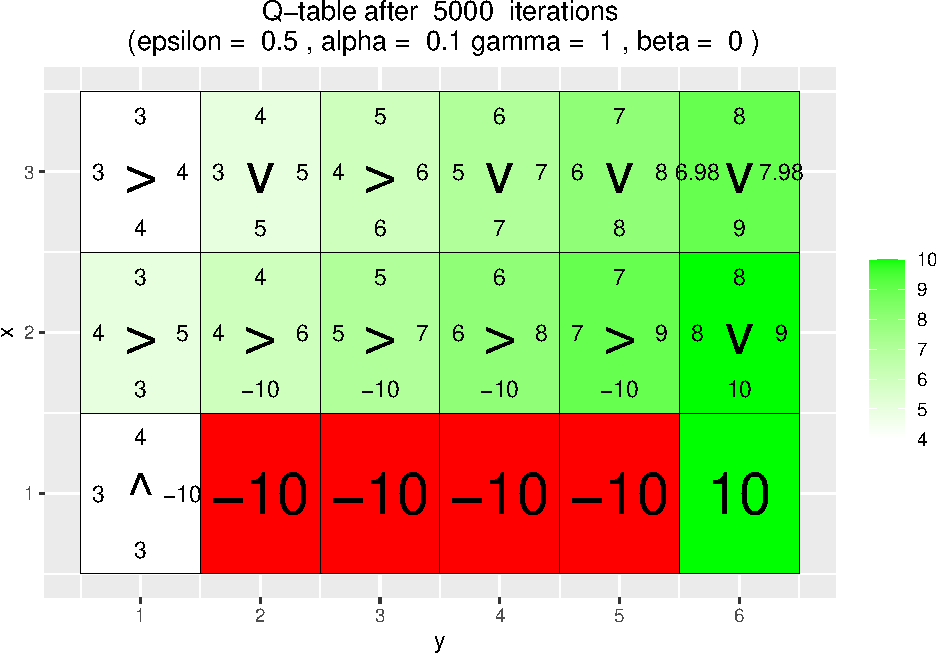
\includegraphics{jan2021_files/figure-latex/unnamed-chunk-3-1.pdf}

\begin{Shaded}
\begin{Highlighting}[]
\DocumentationTok{\#\#\# SARSA }\AlertTok{\#\#\#}
\NormalTok{q\_table }\OtherTok{\textless{}{-}} \FunctionTok{array}\NormalTok{(}\DecValTok{0}\NormalTok{,}\AttributeTok{dim =} \FunctionTok{c}\NormalTok{(H,W,}\DecValTok{4}\NormalTok{))}
\NormalTok{rewardS }\OtherTok{=} \ConstantTok{NULL}
\ControlFlowTok{for}\NormalTok{(i }\ControlFlowTok{in} \DecValTok{1}\SpecialCharTok{:}\DecValTok{5000}\NormalTok{) \{}
\NormalTok{  foo }\OtherTok{\textless{}{-}} \FunctionTok{SARSA}\NormalTok{(}\AttributeTok{epsilon =} \FloatTok{0.5}\NormalTok{, }\AttributeTok{gamma =} \DecValTok{1}\NormalTok{, }\AttributeTok{beta =} \DecValTok{0}\NormalTok{, }\AttributeTok{alpha =} \FloatTok{0.1}\NormalTok{, }\AttributeTok{start\_state =} \FunctionTok{c}\NormalTok{(}\DecValTok{1}\NormalTok{,}\DecValTok{1}\NormalTok{))}
\NormalTok{  rewardS }\OtherTok{=} \FunctionTok{c}\NormalTok{(rewardS,foo[}\DecValTok{1}\NormalTok{])}
\NormalTok{\}}
\FunctionTok{vis\_environment}\NormalTok{(i, }\AttributeTok{epsilon =} \FloatTok{0.5}\NormalTok{, }\AttributeTok{gamma =} \DecValTok{1}\NormalTok{, }\AttributeTok{beta =} \DecValTok{0}\NormalTok{, }\AttributeTok{alpha =} \FloatTok{0.1}\NormalTok{)}
\end{Highlighting}
\end{Shaded}

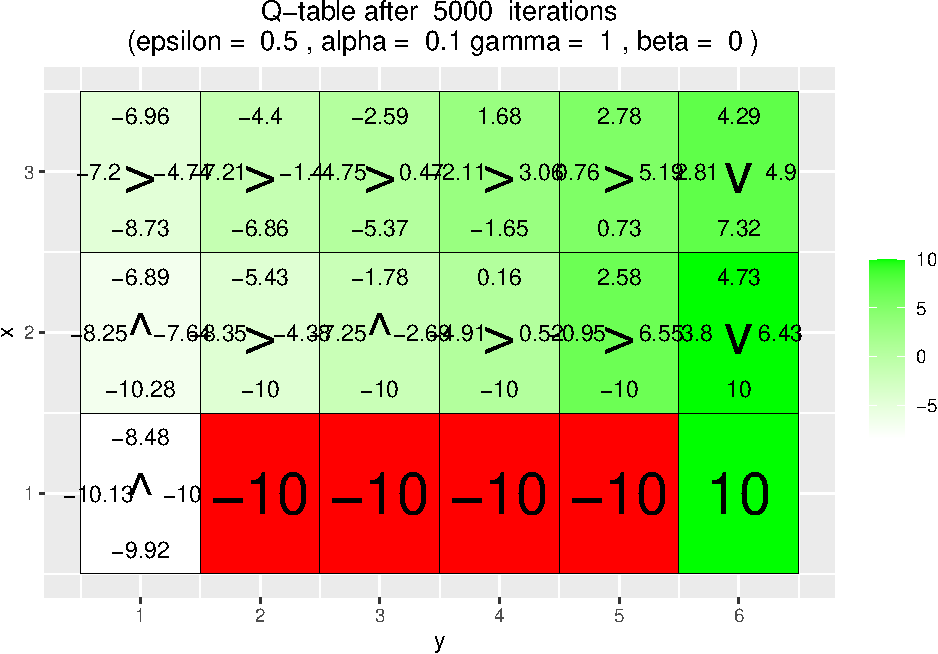
\includegraphics{jan2021_files/figure-latex/unnamed-chunk-3-2.pdf}

\begin{Shaded}
\begin{Highlighting}[]
\DocumentationTok{\#\#\# SARSASA }\AlertTok{\#\#\#}
\NormalTok{q\_table }\OtherTok{\textless{}{-}} \FunctionTok{array}\NormalTok{(}\DecValTok{0}\NormalTok{,}\AttributeTok{dim =} \FunctionTok{c}\NormalTok{(H,W,}\DecValTok{4}\NormalTok{))}
\NormalTok{rewardSA }\OtherTok{=} \ConstantTok{NULL}
\ControlFlowTok{for}\NormalTok{(i }\ControlFlowTok{in} \DecValTok{1}\SpecialCharTok{:}\DecValTok{5000}\NormalTok{) \{}
\NormalTok{  foo }\OtherTok{\textless{}{-}} \FunctionTok{SARSASA}\NormalTok{(}\AttributeTok{epsilon =} \FloatTok{0.5}\NormalTok{, }\AttributeTok{gamma =} \DecValTok{1}\NormalTok{, }\AttributeTok{beta =} \DecValTok{0}\NormalTok{, }\AttributeTok{alpha =} \FloatTok{0.1}\NormalTok{, }\AttributeTok{start\_state =} \FunctionTok{c}\NormalTok{(}\DecValTok{1}\NormalTok{,}\DecValTok{1}\NormalTok{))}
\NormalTok{  rewardSA }\OtherTok{=} \FunctionTok{c}\NormalTok{(rewardSA,foo[}\DecValTok{1}\NormalTok{])}
\NormalTok{\}}
\FunctionTok{vis\_environment}\NormalTok{(i, }\AttributeTok{epsilon =} \FloatTok{0.5}\NormalTok{, }\AttributeTok{gamma =} \DecValTok{1}\NormalTok{, }\AttributeTok{beta =} \DecValTok{0}\NormalTok{, }\AttributeTok{alpha =} \FloatTok{0.1}\NormalTok{)}
\end{Highlighting}
\end{Shaded}

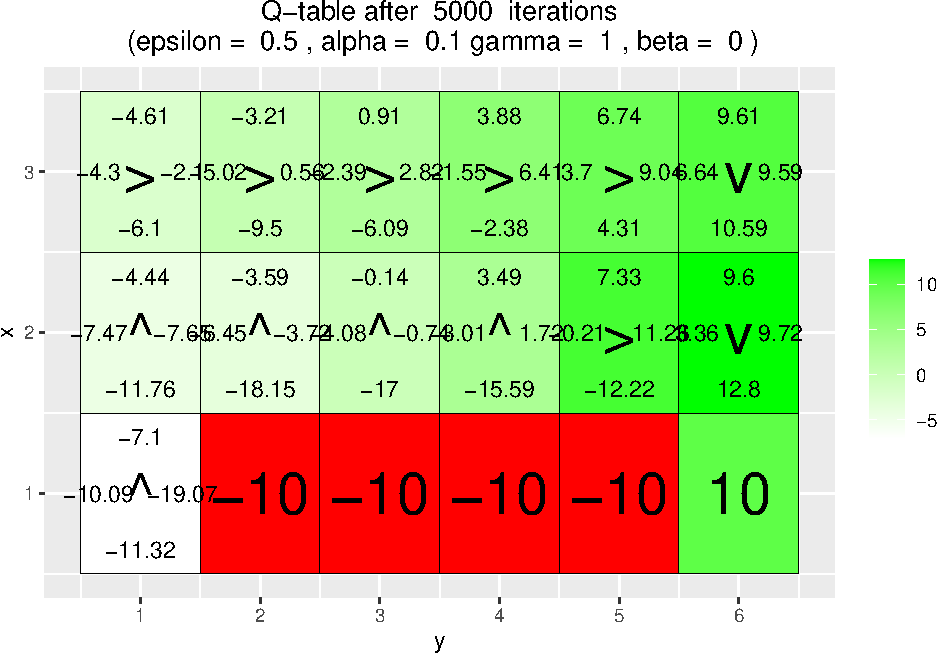
\includegraphics{jan2021_files/figure-latex/unnamed-chunk-3-3.pdf}

\begin{Shaded}
\begin{Highlighting}[]
\FunctionTok{plot}\NormalTok{(}\FunctionTok{MovingAverage}\NormalTok{(rewardQ,}\DecValTok{100}\NormalTok{),}\AttributeTok{type =} \StringTok{"l"}\NormalTok{, }\AttributeTok{col =} \StringTok{"green"}\NormalTok{, }\AttributeTok{ylim =} \FunctionTok{c}\NormalTok{(}\SpecialCharTok{{-}}\DecValTok{15}\NormalTok{,}\SpecialCharTok{{-}}\DecValTok{5}\NormalTok{))}
\FunctionTok{lines}\NormalTok{(}\FunctionTok{MovingAverage}\NormalTok{(rewardS,}\DecValTok{100}\NormalTok{),}\AttributeTok{type =} \StringTok{"l"}\NormalTok{, }\AttributeTok{col =} \StringTok{"blue"}\NormalTok{)}
\FunctionTok{lines}\NormalTok{(}\FunctionTok{MovingAverage}\NormalTok{(rewardSA,}\DecValTok{100}\NormalTok{),}\AttributeTok{type =} \StringTok{"l"}\NormalTok{, }\AttributeTok{col =} \StringTok{"red"}\NormalTok{)}
\end{Highlighting}
\end{Shaded}

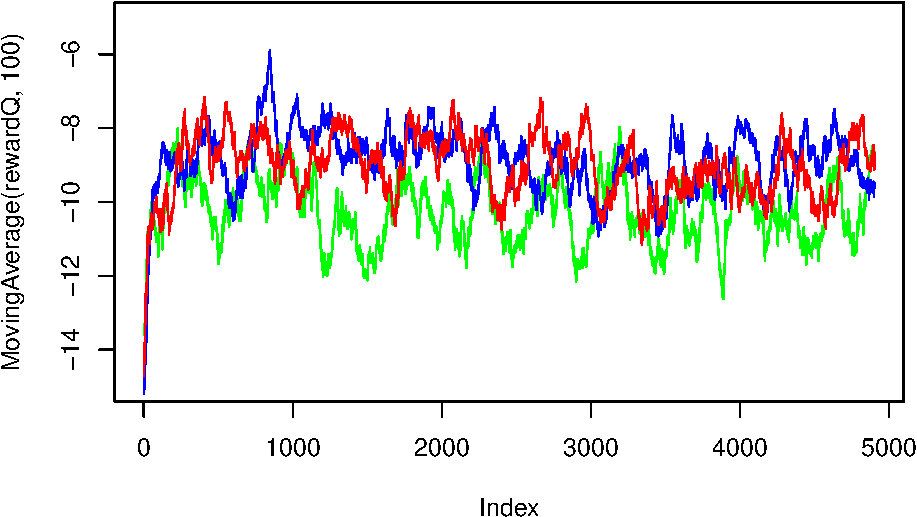
\includegraphics{jan2021_files/figure-latex/unnamed-chunk-3-4.pdf}

\end{document}
